\documentclass{uebblatt}

\begin{document}

\maketitle{2}{-- \emph{Motto} --}

\begin{aufgabe}{Geometrische Realiserung des simplizialen
Standard-$p$-Simplexes}
Wir wollen an einem Beispiel nachvollziehen, dass die Grundlagen
der Theorie der simplizialen Mengen sinnvoll aufeinander abgestimmt sind:
Zeige, dass die geometrische Realisierung~$|\Delta[p]|$ des simplizialen
Standard-$p$-Simplex kanonisch homöomorph zum topologischen
Standard-$p$-Simplex~$\Delta_p$ ist.

Gib dazu explizit die kanonische Abbildung~$|\Delta[p]| \to \Delta_p$ an und
weise nach, dass sie ein Homöomorphismus ist. Später werden wir lernen, wie man
diese Aufgabe auch unmittelbar vermöge abstrakten Nonsens lösen kann.
\end{aufgabe}

\begin{aufgabe}{Fasernde simpliziale Mengen}
Eine simpliziale Menge~$X$ heißt genau dann \emph{fasernd}, wenn für jedes~$n
\geq 0$ und~$k$ mit~$0 \leq k \leq n + 1$ folgende Bedingung erfüllt ist:
\begin{quote}Sind Simplizes~$x_0,\ldots,x_{k-1},x_{k+1},\ldots,x_{n+1} \in X_n$
mit~$d_i x_j = d_{j-1} x_i$ für alle~$i < j$ (wobei~$i$ und~$j$ ungleich~$k$)
vorgegeben, so existiert ein Simplex~$y \in X_{n+1}$ mit~$d_i(y) = x_i$ für
alle~$i \neq k$.
\end{quote}
\begin{enumerate}
\item Was bedeutet diese Bedingung anschaulich? Denke dazu an \emph{Hörner}.
\begin{center}
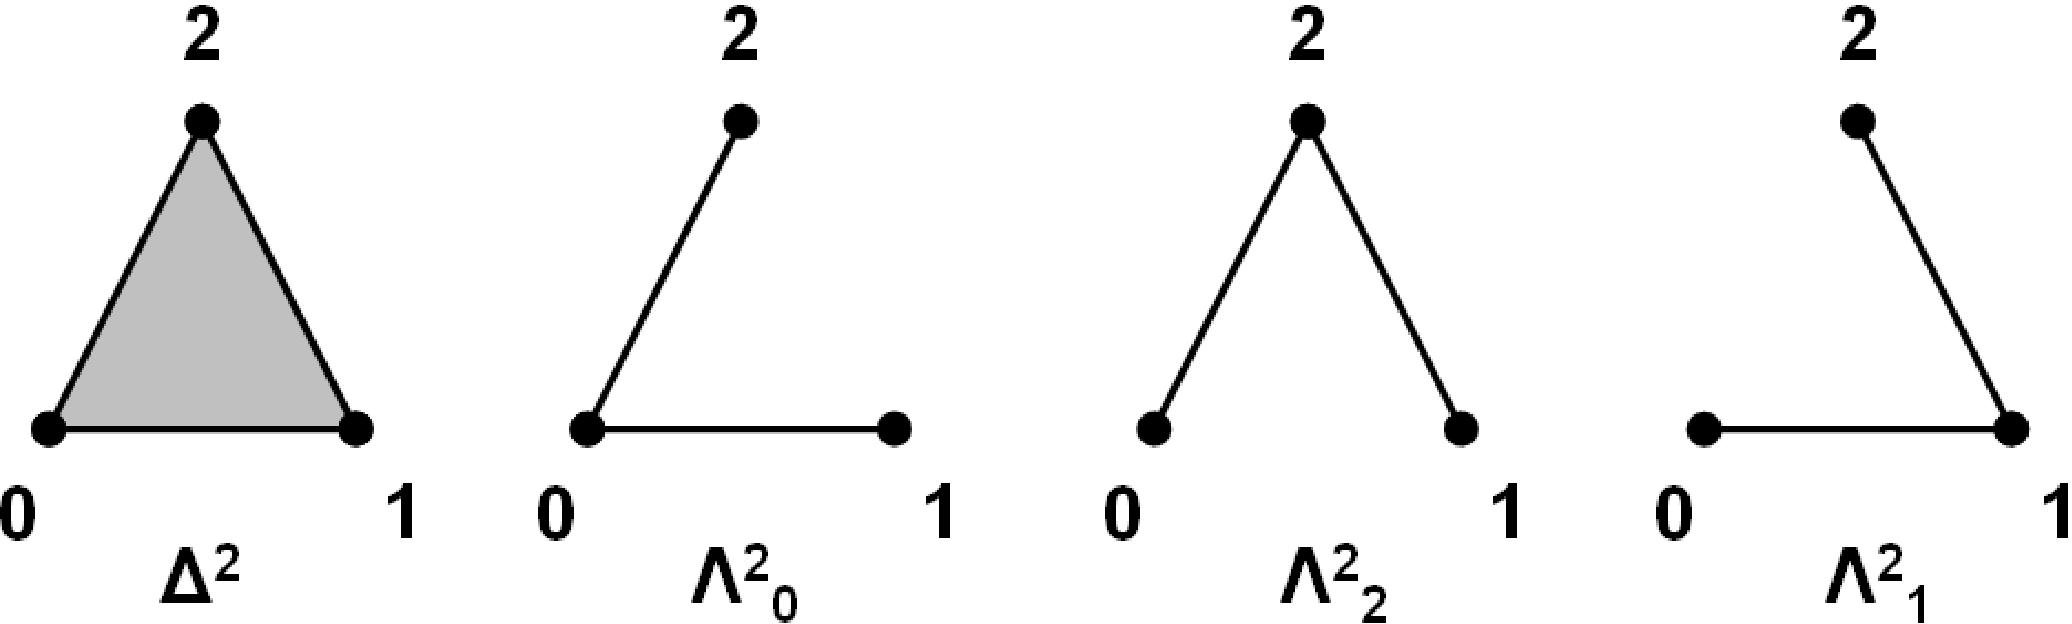
\includegraphics[scale=0.5]{hoerner}

Abbildung: Die drei Hörner von~$\Delta^2$.
\end{center}
\end{enumerate}
\end{aufgabe}

\end{document}
